\documentclass[11pt,dvipdfmx,b5paper,oneside,report,uplatex]{jsbook}


\usepackage{color}
\usepackage{here}
\usepackage{framed}
\usepackage{tcolorbox}
\usepackage{quotchap}
\usepackage{pdfpages}
\usepackage[hidelinks]{hyperref}
\usepackage{pxjahyper}
\usepackage{titlesec}
\usepackage{picture}
\usepackage{tikz}
\usepackage{graphicx}
\usepackage{geometry}
\usepackage{url}
\usepackage{pdfpages}

% 余白を狭くする
\geometry{left=20mm,right=20mm,top=25mm,bottom=25mm}

\tcbuselibrary{breakable,listings}
\definecolor{shadecolor}{gray}{0.80}

% あとがき用のコマンド集
\renewcommand{\textbf}[1]{{\bfseries\sffamily#1}}
\newcommand{\bhline}[1]{\noalign{\hrule height #1}}  

% section
\titleformat{\section}[block]{}{}{0pt}
{
  \definecolor{teal}{gray}{0.30}
  \begin{picture}(0,0)
    \put(-10,-5){
      \begin{tikzpicture}
        \fill[teal] (0pt,0pt) rectangle (5pt,19pt);
      \end{tikzpicture}
    }
    \put(-10,-5){
      \color{teal}
      \line(1,0){\hsize}
    }
  \end{picture}
  \hspace{0pt}
  \sf \Large \thesection
  \hspace{0pt}
}

% 図表見出し
\renewcommand{\tablename}{\textcolor{gray}{▼} 表}
\renewcommand{\figurename}{\textcolor{gray}{▲} 図}

\begin{document}

% タイトル部分
\begin{titlepage}
  \newgeometry{left=0cm,right=0cm,top=0cm,bottom=0cm}
  \centering
  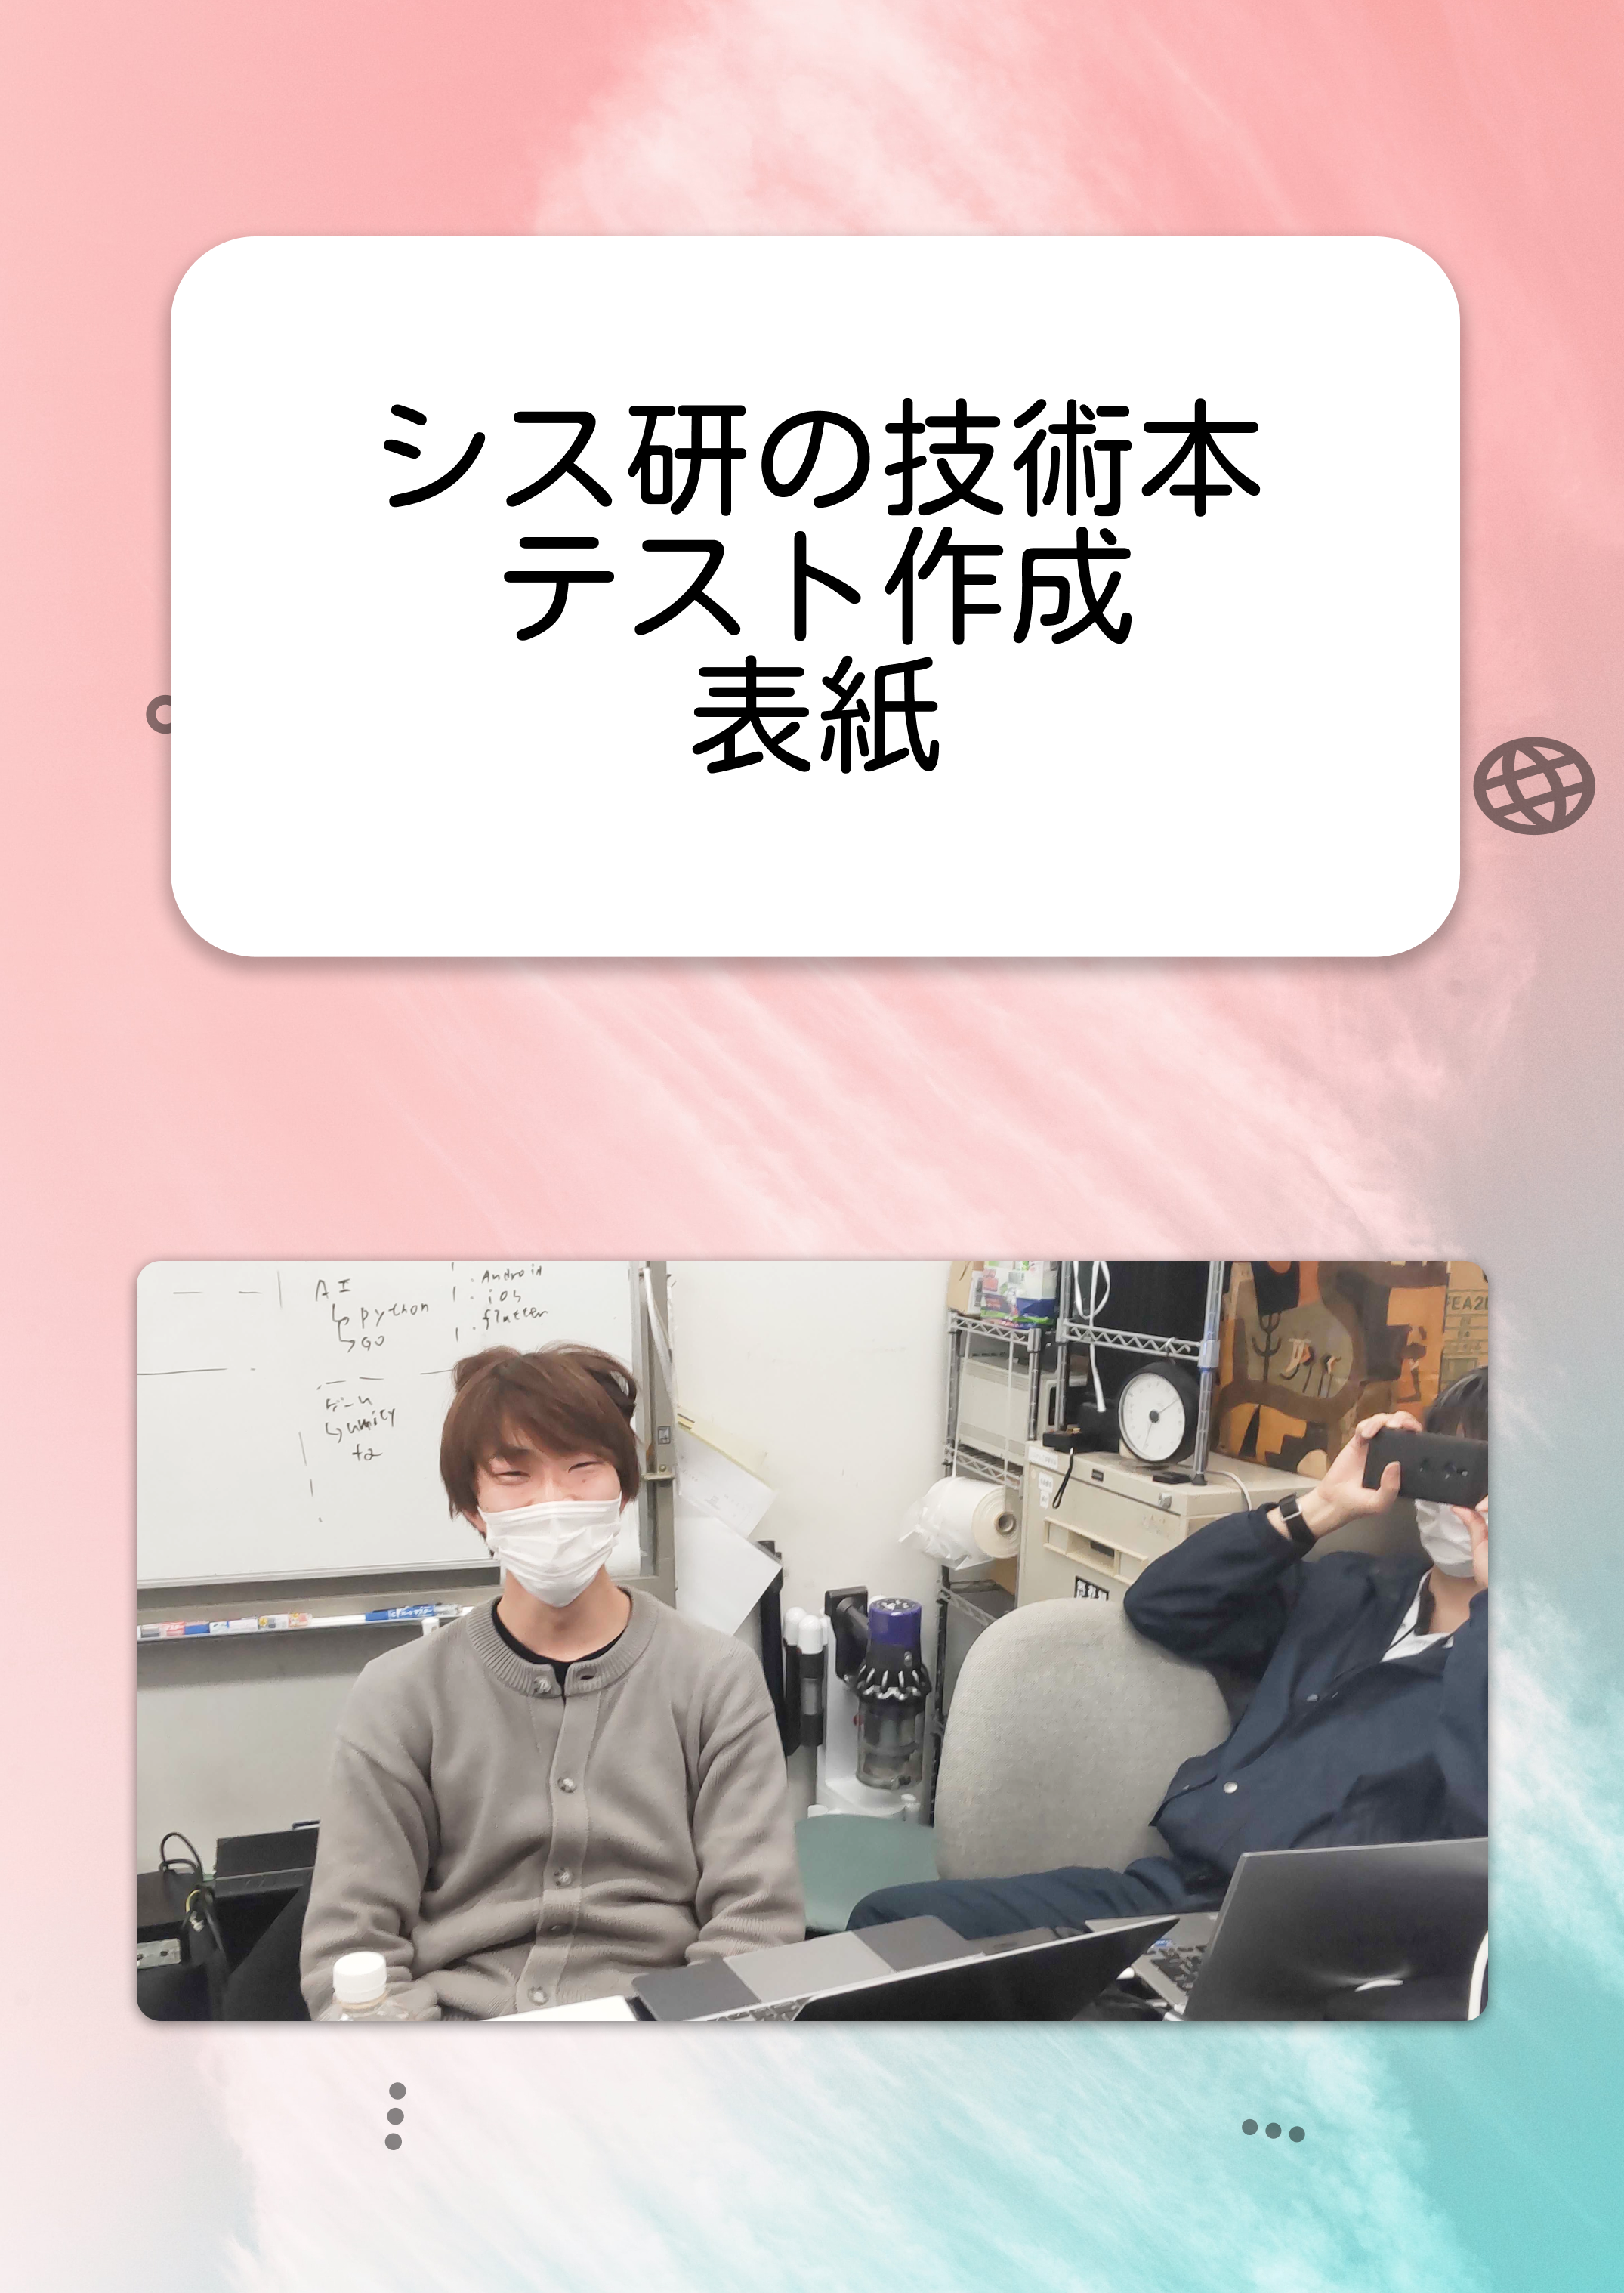
\includegraphics[width=\paperwidth,height=\paperheight]{./image/01-title/titlepage.pdf}
  \restoregeometry % 元の余白に戻す
\end{titlepage}

%目次を自動的に作る。
\tableofcontents

% シス研の紹介
\chapter{シス研というサークルについて}

\section{シス研というサークルについて}
\subsection{はじめに}
初めまして!シス研会長の林です!
はい、ここでみなさんシス研とはなんぞ?となっていると思うのでまずは自分が水先案内人となりましてこの本とシス研について解説していこうと思います。

\subsection{どんな話をするのか}
シス研ってどんなサークル?どんな活動をしているの?この本はどういったもの?といったものを紹介していきます。それでは、さっそく行ってみましょう!!!

\section{シス研とは}
シス研は正式名称を「システム工学研究会」と言い、愛知工業大学公認の情報系サークルです。歴史は長く、2023年で創立47周年を迎え、かのAppleと同い年となります!! \\
シス研ではハッカソン出場をはじめとしたチーム開発、ゲーム作成、インフラの構築、運用などを行っています。

\subsection{どんな活動をしているの?}
シス研の主な活動はチーム開発とインフラ整備です。サークル全体としての開発物などはなく、それぞれがチームを組んでハッカソンに出場したりしています。 \\
インフラ面では、部室に物理サーバを持っており、そこでシス研のホームページや各種サービスを公開しています。\footnote{シス研ホームページ\url{https://set1.ie.aitech.ac.jp}}\footnote{シス研紹介ページ\url{https://welcome.sysken.net}}23年4月現在、大幅な工事を行なっておりごく一部のサービスのみ稼働しています(すみません)
そのほかにもシス研主催のLT会・ハッカソンの開催、Qiitaアドベントカレンダーへの参加もしています。\footnote{Advent Calendar 2022 \url{https://qiita.com/advent-calendar/2022/stech-ait-advent}}

\begin{figure}[bht]
  \centering
  \includegraphics[width=10cm]{./image/02-AboutSysken/room.jpg}
  \caption{部室の様子}
\end{figure}

\subsection{21〜22年度の活動実績}
\begin{itemize}
  \item 2021 愛工大大学祭 工科展 最優秀賞
  \item 2022 技育博 参加
  \item 2022 Geekcamp vol8 優秀賞
  \item 2022 愛工大大学祭 工科展 瑞若賞
  \item 2022 技育展 出展
  \item 2022 愛工大大学祭 模擬店 最優秀賞
  \item 2022 HackU 春・夏 参加
  \item 2022 Geekcampアドバンス 登壇
  \item 長期休暇中のLT会、ハッカソン主催
  \item 各種勉強会の開催
\end{itemize}

\begin{tcolorbox}[title=シス研の設備]
  \begin{itemize}
    \item ブレードサーバ、ネットワーク機器
    \item デスクトップPC
    \item iMac,MacBook
    \item iPhone,iPad
    \item Android端末各種
    \item Raspberry Pi
    \item はんだ等の電子工作セット
    \item その他多数...
  \end{itemize} 
\end{tcolorbox}

\begin{figure}[H]
  \begin{tabular}{cc}
    \begin{minipage}[b]{0.40\columnwidth}
      \centering
      \includegraphics[width=\columnwidth]{./image/02-AboutSysken/server.jpg}
      \caption{ブレードサーバ}
    \end{minipage} &
    \hspace{0.04\columnwidth}
    \begin{minipage}[b]{0.40\columnwidth}
      \centering
      \includegraphics[width=\columnwidth]{./image/02-AboutSysken/network.jpg}
      \caption{ネットワーク機器}
    \end{minipage} \\
    \begin{minipage}[b]{0.40\columnwidth}
      \centering
      \includegraphics[width=\columnwidth]{./image/02-AboutSysken/iPad.jpg}
      \caption{タブレット端末}
    \end{minipage} &
    \hspace{0.04\columnwidth}
    \begin{minipage}[b]{0.40\columnwidth}
      \centering
      \includegraphics[width=\columnwidth]{./image/02-AboutSysken/RaspberryPi.jpg}
      \caption{Raspberry Pi}
    \end{minipage}
  \end{tabular}
\end{figure}

\section{この本について}
この本はシス研のメンバーが経験したこと、取り組んだことのアウトプットを目的としたものです。この本を通じて皆さんにはシス研のメンバーは具体的にどのような活動をしているのか知ってもらいたいと思います。 \\
また、シス研として本を出すのは今回が初めてなのでどうか温かい目で見ていただけると幸いです。

\section{まとめ}
ここまでお話をして来ましたが簡単にでもシス研について知ってもらうことはできたでしょうか?うまく伝えることができていたらとても嬉しいです。 \\
次のページからはメンバーの記事本編になります!シス研初めての本をよろしくお願いします!!

% 技術枠
\chapter{DiscordBotを作ってみよう!}

\section{DiscordBotを作ってみよう}
\subsection{はじめに}
初めに今回何故DiscordのBotを作ろうと思ったかの経緯をお話しします。
私はDiscordで人とチャットをしている時に同じ会話が頻繁に続き、これBotで返事を返すようにしたら返事を返す手間が省けるし面白いのでは?と思ったのがBotを作ろうと思ったきっかけです。
発想がひどいって!?まあでも自分の発想したものを形にすることが面白いことだと思うので今回はそこには目を瞑りましょう…
もちろん自分が送ったメッセージに対してBotに返答させることもできるので、自分だけのオリジナルDiscordBotを作ってみましょう!

\subsection{何を作るのか}
Discordのサーバで特定のメッセージが来たら、特定のメッセージを返すDiscordのBotを作ります。

\section{実行環境・使用技術・ソースコードの管理}
\subsection*{実行環境}
調べる必要あり
\subsection*{使用技術等}
\begin{itemize}
  \item Python(discord.py)を使用
  \item Flaskを用いてWebサーバを構築
\end{itemize}
\subsection*{ソースコードの管理}
\begin{itemize}
  \item Git・GitHubを使用
  \item .envファイルをGitHubにアップロードしないようにする
\end{itemize}

\section{ローカル環境でBotが動作するようにする}
まずはローカル環境でBotが動作するようにしてみます。

\subsection{Botの作成・管理をする}
初めに機能などはまだついていないBotをDiscordのポータルサイトから作成します。
DiscordのBotの作り方(メモ)という記事の「1.Discord上のBotの作成」を見ながらBotを作成してみて下さい。
\footnote{引用した記事についての注釈を書く}。
同記事内の「2.Glitchでサーバーを作成」の部分は、今回Glitchは使用しないため行う必要はありません。

\subsection{Pythonの確認}
先ほど作成したBotをDiscordのサーバーに招待することができたらPythonが使えるかどうかの確認をしましょう。
Pythonを用いて先ほど作成したBotに機能をつけていきます。\\
今回はPythonの3.x系で実装します。\\
まずは、ローカル環境のPythonのバージョンを調べます。\\
\begin{shaded}
\begin{verbatim}
python --version
\end{verbatim}
\end{shaded}
この状態で2.x系のバージョンが出てくる場合は、下記のコマンドで3.x系のバージョンが出てくるか調べます。
\begin{shaded}
\begin{verbatim}
python3 --version
\end{verbatim}
\end{shaded}
今回はPython3.x系を利用するので3.xのバージョンが出たほうで実装を進めてください。\\
また、discord.pyについては3.8以降で動作します。3.8より前のバージョンが表示されている場合は、最新版のPythonをインストールしてください。

\section{本番環境へデプロイする}

\begin{tcolorbox}[breakable]
\begin{verbatim}
1  /* ここにはソースコードを書く */
2  #include<stdio.h>
3
4  int main(void)
5  {
6    printf("Hello, World!\n");
7    return 0;
8  }
9  /* breakableを付けるとこんな感じで改行にも対応できる */
\end{verbatim}
\end{tcolorbox}

\begin{shaded}
\begin{verbatim}
## ここにはコマンドを書く
$ echo "Hello, World!"
\end{verbatim}
\end{shaded}

図表はキャプションを付けたときに、先頭に「▲」や「▼」を付けるようにした。

\begin{table}[H]
  \centering
  \caption{表のサンプル}
  \begin{tabular}{|c|l|l|l|} \hline
    日本 & hoge & fuga & piyo \\ \hline
    アメリカ & foo & bar & baz \\ \hline
  \end{tabular}
  \label{table-sample0301}
\end{table}

\begin{figure}[H]
  \centering
  \includegraphics[width=4cm]{./image/03-Tech/chap1/sample.png}
  \caption{画像のサンプル}
  \label{figure-sample0301}
\end{figure}

\begin{tcolorbox}[title=これはコラム]
  コラムも随時挟めるようにした。

  tcolorboxはtitleを指定するといい感じにタイトル付きの枠で囲ってくれる。
\end{tcolorbox}
\include{./content/03-Tech/section1}
\include{./content/03-Tech/section2}
\lstdefinestyle{mystyle}{
  basicstyle=\ttfamily,
  breakatwhitespace=false,
  breaklines=true,
  keepspaces=true,
}

\section{Gin × Neo4j × Docker で最短経路を返すAPIサーバを建てる}
\subsection{はじめに}
このセクションでは、現在最もメジャーなグラフDBであるNeo4jとGithubでも多くのスターを獲得しているGo言語のWebフレームワーク、Ginを用いて
APIサーバーを構築していきます。また、実行環境統一のためDockerを用います。

\subsection{今回扱うデータの図}
\includegraphics[width=10cm]{./image/03-Tech/chap3/sample_node.png}

\subsection{ディレクトリ構造}
\begin{tcolorbox}[title=ディレクトリ構造]
    \begin{verbatim}
├── build
│   ├── Docker
│   │   ├── go
│   │   │   └── Dockerfile
│   │   └── neo4j
│   │       ├── Dockerfile
│   │       └── volumes
│   │           ├── import
│   │           │   ├── done
│   │           │   ├── points.csv
│   │           │   └── route.csv
│   │           └── script
│   │               └── import_data.sh
│   └── docker-compose.yml
└── server
    ├── config
    │   ├── config.go
    │   └── environments
    │       └── neo4j.yml
    ├── controllers
    │   └── coordinate_controller.go
    ├── db
    │   └── neo4j.go
    ├── go.mod
    ├── go.sum
    ├── main.go
    ├── models
    │   └── coordinate.go
    ├── router
    │   └── router.go
    └── sample.http
\end{verbatim}
\end{tcolorbox}

\subsection{Neo4jに最初にインポートするファイル}

\begin{tcolorbox}[title=point.csv]
    \begin{verbatim}
1 point_id:ID,point_name,:LABEL
2 a,PointA,Point;Position
3 b,PointB,Point;Position
4 c,PointC,Point;Position
5 d,PointD,Point;Position
6 e,PointE,Point;Position
\end{verbatim}
\end{tcolorbox}


\begin{tcolorbox}[title=route.csv]
    \begin{verbatim}
:START_ID,:END_ID,:TYPE,cost:int
b,a,Distance,1
c,b,Distance,3
d,c,Distance,2
e,d,Distance,2
c,a,Distance,1
d,a,Distance,2
e,b,Distance,1
e,a,Distance,1
c,e,Distance,1
d,b,Distance,3
a,b,Distance,1
b,c,Distance,3
c,d,Distance,2
d,e,Distance,2
a,c,Distance,1
a,d,Distance,2
b,e,Distance,1
a,e,Distance,1
e,c,Distance,1
b,d,Distance,3
\end{verbatim}
\end{tcolorbox}
これらをNeo4jにインポートすることで、先ほどの図を表現することができます。
\includegraphics[width=10cm]{./image/03-Tech/chap3/neo4j_result.png}

無事できてますね。

\begin{tcblisting}{title={neo4j.go},listing only,breakable, listing options={style=mystyle}}
  1 version: "3"
  2 services:
  3   go:
  4     container_name: NEO4JAPI_GO
  5     build:
  6       context: ./docker/go
  7       dockerfile: Dockerfile
  8     stdin_open: true
  9     tty: true
  10    volumes:
  11      - ../server:/server
  12    ports:
  13      - 8080:8080
  14    networks:
  15      app_net:
  16        ipv4_address: 192.168.0.1
  17    depends_on:
  18      - "neo4j"
  19
  20  neo4j:
  21    container_name: NEO4JAPI_NEO4J
  22    build:
  23      context: ./Docker/neo4j
  24      dockerfile: Dockerfile
  25    restart: always
  26    ports:
  27      - 57474:7474
  28      - 57687:7687
  29    volumes:
  30      - ./Docker/neo4j/volumes/data:/data
  31      - ./Docker/neo4j/volumes/logs:/logs
  32      - ./Docker/neo4j/volumes/conf:/conf
  33      - ./Docker/neo4j/volumes/import:/import
  34      - ./Docker/neo4j/volumes/script:/script
  35    environment:
  36      - NEO4J_AUTH=neo4j/admin
  37      - EXTENSION_SCRIPT=/script/import_data.sh
  38    networks:
  39      app_net:
  40        ipv4_address: 192.168.0.2
  41
  42 networks:
  43  app_net:
  44    driver: bridge
  45    ipam:
  46      driver: default
  47      config:
  48        - subnet: 192.168.0.0/24
\end{tcblisting}


volumesはデータベースに入れるデータ、ログをバインドするための場所を指定しています。
environmentではユーザーとパスワード、最初に読み込んでもらうシェルスクリプトの場所を指定します。

go関連のDockerfile。
\begin{tcolorbox}[title=Dockerfile]
\begin{verbatim}

1  # goバージョン
2  FROM golang:1.19.3-alpine
3  # アップデートとgitのインストール
4  RUN apk add --update &&  apk add git
5  # appディレクトリの作成
6  RUN mkdir /server
7  # ワーキングディレクトリの設定
8  WORKDIR /server
9  # ホストのファイルをコンテナの作業ディレクトリに移行
10 ADD . /server
11 # main.goを実行
12 CMD ["go", "run", "main.go"]
\end{verbatim}
\end{tcolorbox}

Neo4j関連のDockerfile。
\begin{tcolorbox}[title=Dockerfile]
\begin{verbatim}
1  # goバージョン
2  FROM golang:1.19.3-alpine
3  # アップデートとgitのインストール
4  RUN apk add --update &&  apk add git
5  # appディレクトリの作成
6  RUN mkdir /server
7  # ワーキングディレクトリの設定
8  WORKDIR /server
9  # ホストのファイルをコンテナの作業ディレクトリに移行
10 ADD . /server
11 # main.goを実行
12 CMD ["go", "run", "main.go"]
\end{verbatim}
\end{tcolorbox}

csvファイルを読ませるためのシェルスクリプト。
\begin{tcolorbox}[title=import\_data.sh]
\begin{verbatim}
1  #!/bin/bash
2  set -euC
3
4  # EXTENSION_SCRIPTはコンテナが起動するたびにコールされるため、
5  # import処理が実施済かフラグファイルの有無をチェック
6  if [ -f /import/done ]; then
7      echo "Skip import process"
8      return
9  fi
10
11 # データを全削除
12 echo "delete database started."
13 rm -rf /data/databases
14 rm -rf /data/transactions
15 echo "delete database finished."
16
17 # CSVデータのインポート
18 echo "Start the data import process"
19 neo4j-admin import \
20   --nodes=/import/points.csv \
21   --relationships=/import/route.csv
22 echo "Complete the data import process"
23
24 # import処理の完了フラグファイルの作成
25 echo "Start creating flag file"
26 touch /import/done
27 echo "Complete creating flag file"
\end{verbatim}
\end{tcolorbox}
    
\subsection{Goのソースコード}
\subsubsection{configディレクトリ}

\begin{tcolorbox}[title=config.go]
\begin{verbatim}
1  package config
2
3  import (
4  	  "github.com/spf13/viper"
5  )
6
7  var n *viper.Viper
8
9  func init() {
10 	 n = viper.New()
11	 n.SetConfigType("yaml")
12 	 n.SetConfigName("neo4j")
13 	 n.AddConfigPath("config/environments/")
14 }
15
16 func GetNeo4jConfig() *viper.Viper {
17	 if err := n.ReadInConfig(); err != nil {
18		 return nil
19	 }
20	 return n
21 }
\end{verbatim}
\end{tcolorbox}
このファイルでneo4j.yamlの環境変数を読み込みます。
\begin{tcolorbox}[title=neo4j.yml]
\begin{verbatim}
1 neo4j:
2  user: neo4j
3  password: admin
4  uri: neo4j://192.168.176.1:57687
\end{verbatim}
\end{tcolorbox}
Neo4jと接続するための環境変数です。

\subsubsection{dbディレクトリ}





\begin{tcblisting}{title={neo4j.go},listing only,breakable, listing options={style=mystyle}}
1  package db
2
3  import (
4   "log"
5
6   "neo4japi/server/config"
7
8   "github.com/neo4j/neo4j-go-driver/v4/neo4j"
9  )
10
11 func GetDriverAndSession() neo4j.Session {
12   n := config.GetNeo4jConfig()
13   dr, err := neo4j.NewDriver(n.GetString("neo4j.uri"), neo4j.BasicAuth(n.GetString("neo4j.user"), n.GetString("neo4j.password"), ""))
14   if err != nil {
15     log.Fatal(err)
16   }
17   ses := dr.NewSession(neo4j.SessionConfig{AccessMode: neo4j.AccessModeRead})
18   return ses
19 }
  \end{tcblisting}
  
このファイルでNeo4jと接続し、セッションを返すようにします。
\subsubsection{modelsディレクトリ}


\begin{tcblisting}{title={coordinate.go},listing only,breakable, listing options={style=mystyle}}
  1  package models
  2
  3  import (
  4   "fmt"
  5   "log"
  6
  7   "neo4japi/server/db"
  8
  9   "github.com/neo4j/neo4j-go-driver/v4/neo4j"
  10 )
  11
  12 type Route struct {
  13   Position string `json:"point"`
  14 }
  15
  16 func FindRoute(fr, to string) []*Route {
  17   var r []*Route
  18   ses := db.GetDriverAndSession()
  19   defer ses.Close()
  20   cyp := fmt.Sprintf(`
  21     MATCH (from:Position {point_name: "%s"}), (to:Position {point_name: "%s"}), 
  22       path=allShortestPaths ((from)-[distance:Distance*]->(to))
  23     WITH
  24       [position in nodes(path) | position.point_name] as name,
  25     REDUCE(totalMinutes = 0, d in distance | totalMinutes + d.cost) as 所要時間
  26     RETURN name
  27     ORDER BY 所要時間
  28     LIMIT 10;
  29   `, fr, to)
  30
  31   _, err := ses.ReadTransaction(func(transaction neo4j.Transaction) (interface{}, error) {
  32     result, err := transaction.Run(cyp, nil)
  33     if err != nil {
  34       return nil, err
  35     }
  36     if result.Next() {
  37       name, _ := result.Record().Get("name")
  38       nameAr := name.([]interface{})
  39
  40       for i := 0; i < len(nameAr); i++ {
  41         r = append(r, &Route{nameAr[i].(string)})
  42      }
  43     }
  44     return nil, result.Err()
  45   })
  46   if err != nil {
  47     log.Fatal(err)
  48   }
  49   return r
  50 }
    \end{tcblisting}



出発地点と目的地を受け取ることでNeo4jにCypherというクエリ言語を用いて最短経路を導出してもらいます。
\subsubsection{controllersディレクトリ}

\begin{tcolorbox}[title=coordinate\_controller.go]
\begin{verbatim}
1  package controllers
2
3  import (
4	  "net/http"
5
6	  "github.com/gin-gonic/gin"
7	  "neo4japi/server/models"
8  )
9
10 func RouteSearch(c *gin.Context) {
11	 fr := c.Query("fr")
12	 to := c.Query("to")
13	 res := models.FindRoute(fr, to)
14	 c.JSON(http.StatusOK, res)
15 }
\end{verbatim}
\end{tcolorbox}
GETリクエストで受け取ったパラメータを models で作成した関数に渡します。
\subsubsection{routerディレクトリ}

\begin{tcolorbox}[title=router.go]
\begin{verbatim}
1  package router
2
3  import (
4	  "github.com/gin-gonic/gin"
5	  "neo4japi/server/controllers"
6  )
7
8  func Init() {
9	  r := gin.Default()
10	 r.GET("/coordinate", controllers.RouteSearch)
11	 r.Run()
12 }
\end{verbatim}
\end{tcolorbox}
ルーティング先を定義します。
\subsubsection{実行ファイル}
\begin{tcolorbox}[title=coordinate\_controller.go]
\begin{verbatim}
1  package main
2
3  import (
4	  "neo4japi/server/router"
5  )
6
7  func main() {
8	  router.Init()
9  }
\end{verbatim}
\end{tcolorbox}

\subsection{実行方法}
\begin{tcolorbox}[breakable]
\begin{verbatim}
docker compose up
\end{verbatim}
\end{tcolorbox}
このコマンドを実行することで Neo4j サーバーと Gin サーバーが立ち上がります。
\subsubsection{実行確認}

\begin{tcolorbox}[title=sample.http]
\begin{verbatim}
1  GET http://localhost:8080/coordinate?fr=PointB&to=PointE
\end{verbatim}
\end{tcolorbox}
今回はVSCodeの拡張機能であるREST Clientを用いて実行確認を行います。

ここで、 coordinate?fr=PointB\&to=PointE の部分を自分の好きな地点にしてリクエストを送ると、最短経路が返されます。

\subsection{おわりに}
このチャプターではグラフDBとGo言語を用いたAPIサーバーの建て方を説明しました。
Gin、Neo4jは奥が深いので、もし気になった方はぜひ自分で調べて触ってみてください。

\include{./content/03-Tech/section4}

% 日常枠
\chapter{シス研の日常}

シス研は技術一辺倒ではなく、次のような活動をしているメンバーもいます!

\begin{tcolorbox}[title=お品書き]
  \begin{itemize}
    \item p.47『戦闘機に乗ろう』松土
          戦闘機のフライトシュミレータの紹介をしています!
  \end{itemize} 
\end{tcolorbox}

\begin{figure}[H]
  \centering
  \includegraphics[width=6cm]{./image/04-Intarasting/takoyaki_soryusyon.jpg}
  \caption{たこ焼きでITをそりゅーしょんしている様子}
  \label{takoyaki_soryusyon}
\end{figure}
\include{./content/04-Intarasting/section1}
\include{./content/04-Intarasting/section2}

% 奥付け
% TODO: chapterやsectionは適宜修正お願い
\chapter{あとがき枠}

\section{本誌創刊に寄せて}

物は試し、ということわざがあります。
また、言うは易く行なうは難し、ということわざもあります。
どちらのことわざにしても、実際にやってみれば良く分かる、という共通の帰結があります。
しかし、あまりに簡単に実行できる仕組みを作ってしまうと、しばしば人間は仕組み無しで試すことや仕組み自体を軽視し始め、その仕組みの存在のありがたさを忘れてしまうものなのでしょう。
そして、失って初めてその存在のありがたみに気が付く、という言葉は、前述のような体験を経た (やってみた) 人からしばしば生まれてくる言葉なのでしょう。
では、あまりに簡単に成功する仕組みがある状況下で、次代にその仕組みの意味や価値を伝えるにはどうすればよいのでしょうか。

次代の人々に対して、比較的短期間かつ効果が期待できる方法のひとつに、意図的な損失を生み出す方法があります。
失って気が付くのであれば一度失ってみさせれば良い、という考えです。
しかし、一度得たものを失うことに少なからず不満を抱いてしまうのは、人間の性です。
故に、実行者にはその不満の矛先が向けられる可能性があります。
また、損失は発展を阻害する要因でもあります。
従って、進歩のための損失であるように、損失の度合いには十分に配慮しなければなりません。

一方で、正義は常に正しいとは限らない、という考えがあります。
それは、時代や地域や環境によって、文化や思想や理念など、是非を判断する上での前提条件が異なるからです。
ある正義の下では正当だとされる仕組みでも、別の正義の下では不当だとされ得るということです。
しかしながら、正義は人間の行為における動機付けのひとつとされています。
昨日までの正義を否定するような今日の正義に直面した時、我々はどのように受け止め考えていけば良いのでしょうか。
選択肢として、一切の拒絶をするか、昨日までの自らの行いを否定することによって自己正当化をするか、などが考えられます。
それらの中でも、多少なりとも理解を試み受け入れようとする選択が、多角的な視点からより良い考えが期待できるでしょう。

私はシス研に長らく在籍していました。
本誌のような試みが10年振りに復活し、製本されることを大変嬉しくありがたく思っています。
シス研では、ある時は観察者として、またある時は友や助言者として、そして敵として、振舞いました。
かつて理想と信念を掲げ、仲間と共にある時代を築いた者のひとりとして、自主的に行ったとはいえ、次代の芽が出るまでの橋渡し役はなかなかに堪えるものでした。
自らが信じた正義と次代を担う彼らの正義を常に見比べ、その上で役割を果たす必要があったからです。
何かを手に入れようとする若さを生かすためには、何かを失うまいとする老いた私情は捨て去らねばなりません。
しかしながら、過去の歴史を知り同じ過ちを繰り返さないようにすることは、未来を思い描くために重要なことであるはずです。
ある意味ではそれを正義として、客観的な答えを導くために私は自分自身を自制していたのかもしれません。
少なくとも、未来を思い描く先導者にとって、彼ら自身が追従するような相手はいませんから。

これから、シス研は新たな時代を迎えようとしています。
最後に、マハトマ・ガンジーが残した2つの名言で締めつつ、シス研の今後の活動にご期待ください。

\begin{quote}
    物事は初めはきまって少数の人によって、ときにはただ一人で始められるものである。
    \\
    満足は努力の中にあって、結果にあるものではない。
\end{quote}

\newpage
\thispagestyle{empty}
\section*{奥付け}

\begin{table}[b]%
	\centering%
	\begin{tabular}{lcll}%
		\multicolumn{4}{c}{ {\LARGE Syskenの技術本 様々な技術を詰め合わせてみました。} }	\\
		\bhline{1pt}
		発行日 && 2023年 5月 28日 & (初版)	\\
%		 && 2019年 $\phantom{1}$2月 28日 &	(第二版)\\
		サークル && 愛知工業大学 システム工学研究会 &	\\
    Instagram ID && @ait.sysken& 	\\
		Twitter ID && @set$\_$official &	\\
		QiitaOrganizationURL && https://qiita.com/organizations/sysken &	\\
		代表 && 牧野遥斗 & \\
		代表者メールアドレス && harutiro2027@icloud.com & \\
		企画・編集 && 牧野遥斗 (Twitter: @minesu1224)  &	\\
		著者 && 林航平  &	\\
		   && すださんかり  &	\\
		   && hihumikan  &	\\
		   && Beyond Toyama  &	\\
		   && 水谷祐生 (Twitter @l8ZAFNZbON1eDbZ)  &	\\
		   && BlacKnight松土 (Twitter:@kk22blacknight)  &	\\
		   && shirataki1126  &	\\
		印刷所 && しまや出版 & \\
		\bhline{1pt}
		\multicolumn{4}{c}{ {※本書の無断複写、複製、データ配信はかたくお断りいたします。} }	
	\end{tabular}%
\end{table}%



\end{document}